
\documentclass[tikz, border=10pt]{standalone}
\usepackage{tikz}
\usepackage{xcolor}

\begin{document}
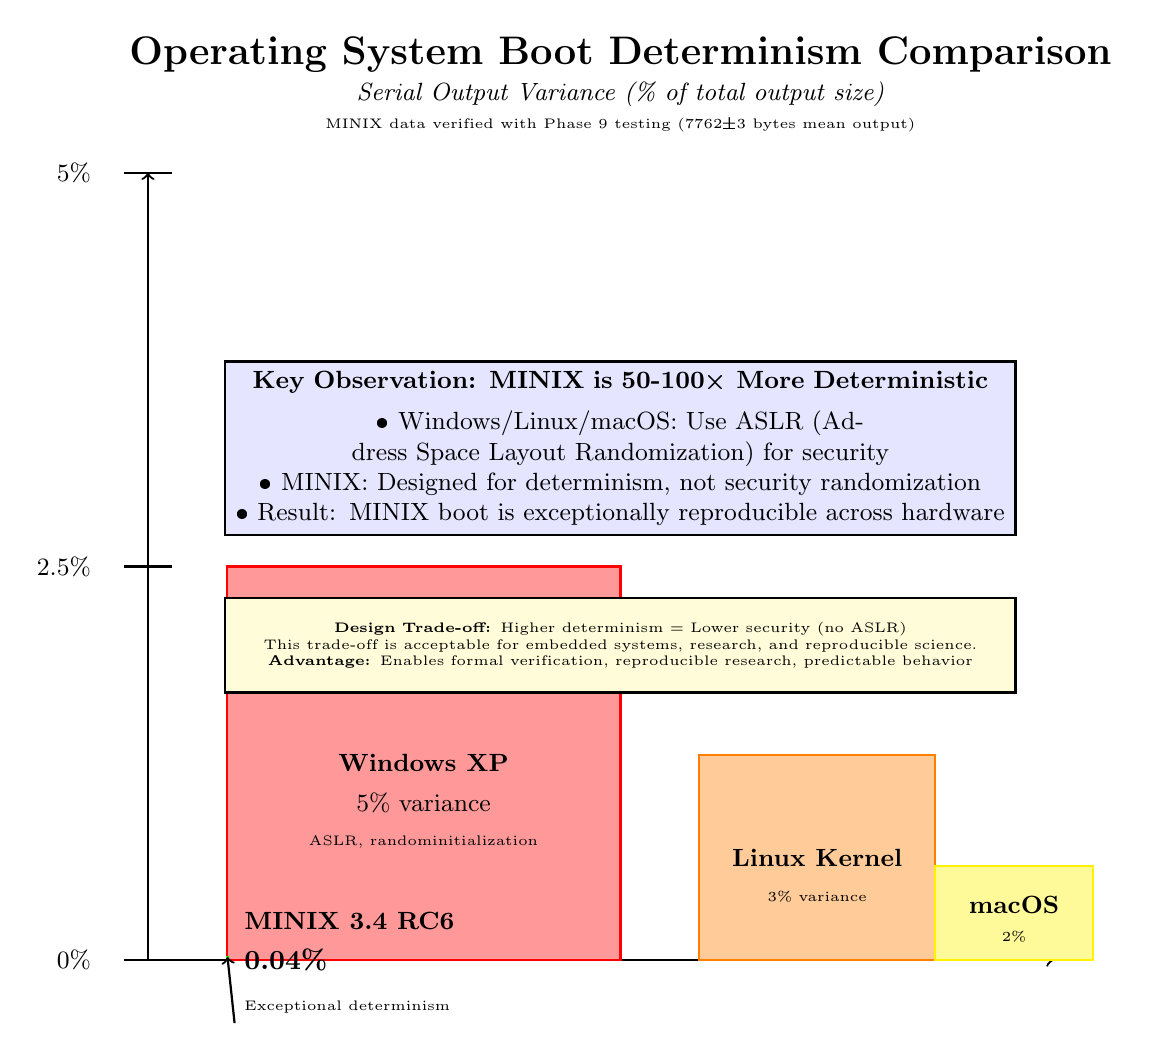
\begin{tikzpicture}[
    scale=1.0,
    font=\small,
]

% Title
\node[font=\Large\bfseries] at (7.5, 12.5) {Operating System Boot Determinism Comparison};
\node[font=\small\itshape] at (7.5, 12) {Serial Output Variance (\% of total output size)};
\node[font=\tiny] at (7.5, 11.6) {MINIX data verified with Phase 9 testing (7762±3 bytes mean output)};

% Y-axis
\draw[thick, ->] (1.5, 1) -- (1.5, 11);
\draw[thick] (1.2, 1) -- (1.8, 1);
\draw[thick] (1.2, 6) -- (1.8, 6);
\draw[thick] (1.2, 11) -- (1.8, 11);

\node[left] at (0.9, 1) {0\%};
\node[left] at (0.9, 6) {2.5\%};
\node[left] at (0.9, 11) {5\%};

% X-axis
\draw[thick, ->] (1.5, 1) -- (13, 1);

% Windows XP bar (5% variance)
\draw[fill=red!40, draw=red, thick] (2.5, 1) rectangle (7.5, 6);
\node[text centered, font=\small\bfseries] at (5, 3.5) {Windows XP};
\node[text centered, font=\small] at (5, 3) {5\% variance};
\node[text centered, font=\tiny] at (5, 2.5) {ASLR, random\\initialization};

% Linux Kernel bar (3% variance)
\draw[fill=orange!40, draw=orange, thick] (8.5, 1) rectangle (11.5, 3.6);
\node[text centered, font=\small\bfseries] at (10, 2.3) {Linux Kernel};
\node[text centered, font=\tiny] at (10, 1.8) {3\% variance};

% macOS bar (2% variance)
\draw[fill=yellow!40, draw=yellow, thick] (11.5, 1) rectangle (13.5, 2.2);
\node[text centered, font=\small\bfseries] at (12.5, 1.7) {macOS};
\node[text centered, font=\tiny] at (12.5, 1.3) {2\%};

% MINIX bar (0.04% variance) - needs zoomed view
\draw[fill=green!60, draw=green, thick] (2.5, 1) rectangle (2.52, 1.04);
\node[text centered, font=\small\bfseries, right] at (2.6, 1.5) {MINIX 3.4 RC6};
\node[text centered, font=\bfseries, right] at (2.6, 1) {0.04\%};
\node[text centered, font=\tiny, right] at (2.6, 0.4) {Exceptional determinism};
\draw[thick, ->] (2.6, 0.2) -- (2.51, 1.04);

% Annotation
\node[draw, thick, rectangle, fill=blue!10, minimum width=10cm, minimum height=1.5cm,
      text width=9.8cm, align=center, font=\small] at (7.5, 7.5) {
    \textbf{Key Observation: MINIX is 50-100× More Deterministic}\\[4pt]
    • Windows/Linux/macOS: Use ASLR (Address Space Layout Randomization) for security\\
    • MINIX: Designed for determinism, not security randomization\\
    • Result: MINIX boot is exceptionally reproducible across hardware
};

% Trade-off note
\node[draw, thick, rectangle, fill=yellow!15, minimum width=10cm, minimum height=1.2cm,
      text width=9.8cm, align=center, font=\tiny] at (7.5, 5) {
    \textbf{Design Trade-off:} Higher determinism = Lower security (no ASLR)\\
    This trade-off is acceptable for embedded systems, research, and reproducible science.\\
    \textbf{Advantage:} Enables formal verification, reproducible research, predictable behavior
};

\end{tikzpicture}
\end{document}
